\section{Introduction}

Few of the products and services we use on a daily basis occur naturally within our environment. Most all of them are the result of some concerted effort of individuals to provide those products and servivces. This production process can take many forms, and comprise numerous different processing steps. Oftentimes, these steps can involve multiple independent organizations working in concert with one another.

Operations management is the area of business specialization that focuses on the value creation, on how the products and services we consume each day are created. However, this is clearly not all the activities in which businesses engage. Corporations are involved in financial management activities, contract negotiations and legal proceedings, strategy planning, the development of new products, the marketing of products, hiring new talent, training of staff, and numerous other functions necessary to keep the business functioning properly.

The goal of this paper is to analyze the various components of operations management in relationship to organizational success. Of necessity, this discussion will lack some specificity as differing organizations will need different types of operations management. For example, a cloud-based internet services company will not have a need for any manufacturing facilities, and IT functions will be part of operations. By contrast, a traditional manufacturing company will have significant manufacturing facilities under operational control, while IT may well be outside the scope of operations and instead be considered a support function. A third option, represented by the rise of ``Industry 4.0'' companies could have IT as part of operations while the actual manufacturing function is an outsourced service \parencite{gasparImpactsIndustryOperations2020}.

At it's most basic level, operations recieves inputs, utilizes a repeatable process to transform those inputs, and produces outputs (fig \ref{fig:basic}).

\begin{minipage}{\linewidth}
  \makebox[\linewidth]{ % to center image}
    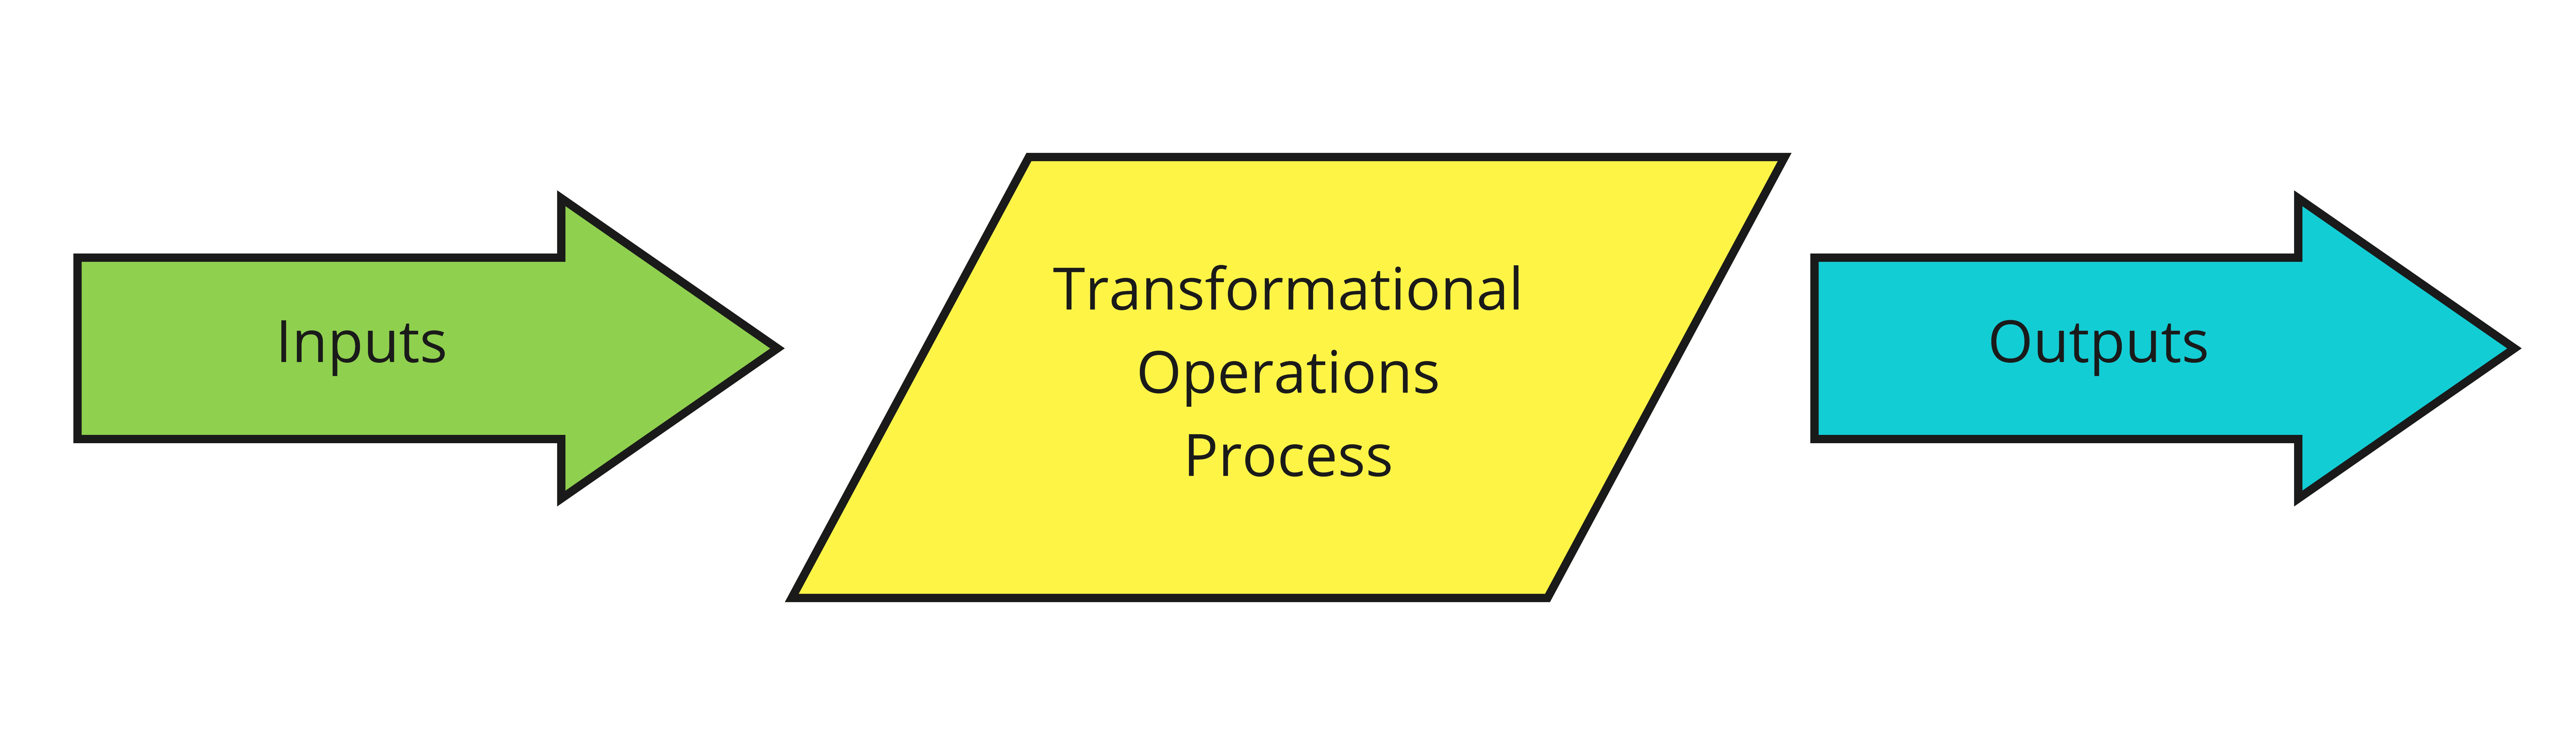
\includegraphics[width=6in]{img/basic}}
    \captionof{figure}{Basic Operations}
    \label{fig:basic}
\end{minipage}

Of course, for any organization of any scale, there needs to be feedback from the outputs to the new inputs to allow for improvements and to ensure the effficacy and quality of the transformational process.

It is the purpose of this paper to examine how the transforamtional process and feedback loops that allow inputs to become outputs fits within the broader context of an organization.
